\documentclass[a4paper, 11pt]{exam}
\usepackage{titling}
\newcommand{\subtitle}[1]{%
  \posttitle{%
    \par\end{center}
    \begin{center}\large#1\end{center}
    }%
}

\usepackage{url}
\usepackage{amsmath,amsthm,enumitem,amssymb}
\usepackage{graphicx}
\usepackage{hyperref}
\renewcommand{\labelenumii}{\roman{enumii}}

\title{Homework Assignment 2}
\subtitle{CS/ECE 6810: Computer Architecture \\
Jan 31,2018 \\
Maryam Dabaghchian-u1078006}

\author{ \\
\textbf{Pipelining}}
\date{Due Date: Feb 13, 2018.\\
90 points}

\begin{document}
\maketitle
\begin{center}
\fbox{\fbox{\parbox{5.9in}{\centering
Important Notes:
\begin{itemize}
\item Solutions turned in must be your own. Please, mention references (if any) at the end of each question. Please refrain from cheating.
\item All solutions must be accompanied by the equations used/logic/intermediate steps. Writing only the final answer will receive \textbf{zero} credit.
\item All units must be mentioned wherever required.
\item Late submissions \textbf{(after 11:59 pm on 02/13/2018)} will not be accepted
\item All submissions must be in PDF only. Scanned copies of handwritten solutions will not be accepted as a valid submission.
\end{itemize}
}}}
\end{center}
\vspace{0.2in}

\begin{enumerate}
	\item \textbf {Pipelining Performance}
    Consider a single-cycle processor in which the execution of
every instruction completes in 10 ns. The goal is to execute a user application that consists of 1000 instructions.
	\begin{enumerate}
    \item If the single cycle processor can execute one instruction per cycle, find the CPU time. \textbf{(5 points)}
    
\fbox{\parbox{5.5in}{
    \textbf{Answer}
    \vspace{0.2in} 
	According to the assumption, the processor is single-cycle and every instruction completes in 10$^{ns}$, so $CT = 10^{ns}, IPC = 1$. In the unpipelined case, all instructions are completed sequentially, so the total CPU time would be as follows:
	$$
	Time = IC \times CPI \times CT = 1000 \times 1 \times 10 = 10000^{ns}
    $$
    }}
    \newline
    
   
    \item Assuming a 1ns additional delay for pipeline registers and perfect circuit partitioning and pipelining, find the speedup gained by making the processor 10- stage pipelined. Assume that 2 bubbles (NOPs) are necessary every 10 cycles for load and branch instructions. \textbf{(15 points)}
    
\fbox{\parbox{5.5in}{
    \textbf{Answer}
    \vspace{0.2in} 
     According to the previous part, every instruction takes $T=10^{ns}$ to complete. 
     So, in a $N=$10-stage pipeline, with $T_{ovh} = 1^{ns}$ delay time per stage, the 
     total time per stage would be:
     $$
     Time_{stage} = \frac{T}{N} + T_{ovh} = \frac{10}{10} + 1 = 2^{ns}.
     $$
     Considering 2 bubble per 10 cycle, every instruction would complete in 12 stages:
     $$
     Time_{instruction} = \frac{12}{10} \times Time_{stage} = 2.4^{ns}.
     $$
     Finally, the total CPU time in the pipeline would be:
     $$
     Time_{pipeline} = 1000 \times Time_{instruction} = 2400^{ns}.
     $$
     On the other hand, for the unpipeline case, the cpu time would be:
     $$
     Time^{unpipe}_{instruction} = T + T_{ovh} = 10 + 1 = 11
     $$
     $$
     Time_{unpipeline} = 1000 \times Time^{unpipe}_{instruction} = 11000^{ns}.
     $$
     
     Therefore, the speedup is gained as follows.
	 $$
     speedup = \frac{Time_{unpipeline}}{Time_{pipeline}} = 
     \frac{11000}{2400} = 4.58
     $$
    }}
	\newline
    
	\end{enumerate}
    
    \item \textbf{Control Hazards} Consider an in-order five-stage pipeline that determines the branch
target by the end of the 3rd pipeline stage (i.e., the execute stage). To avoid branch related stalls, the instruction set architecture (ISA) defines two branch delay slots. Assume that (a) all stalls in the processor are branch-related, (b) $20\%$ of all instructions are branches, (c) a branch is taken $60\%$ of the time, and (d) you could move two instructions from the taken side into the branch delay slot. What is the expected CPI for
this processor? \textbf{(15 points)} 

\fbox{\parbox{5.8in}{
    \textbf{Answer}
    \vspace{0.2in} 
    According to the assumptions, the number of branch instructions is $20\%$ of the 
    total instruction count. In addition, all stalls are related to branch instructions, and in 
    60\% of the time a branch is taken, in which case two instruction of the taken side 
    could be moved into the branch slot (i.e. we can consider no delay when a branch is 
    taken, and branch slot takes two cycles). Therefore, for 60\% of branches, i.e., 
    12\% ($0.6 \times 0.2$) plus 80\% of the instructions, there is no delay. Since we 
    have a 5-stage pipeline, for instructions without any delay, i.e., $92\%$ of 
    instructions, CPI would be $1$. And each branch instructions with delay, i.e., 
    $8\% (0.4 \times 0.2)$ of the instructions, will complete in 3 cycles with respect 
    to 2 stalls. Therefore, CPI would be as follows.
$$
CPI = 0.92 + (3 \times 0.08) = 1.16.
$$

    }}
	\newline
    
	\item \textbf{Multi-cycle Instructions} A pipelined architecture comprises instruction fetch (IF), instruction issue (IS), register read (RR), execute (EX), and write-back (WB) stages. Except EX, each stage requires one clock cycle to complete. The EX stage includes 4
functional units, each of which can perform a floating-point operation —e.g., ADD, SUB, MULT, DIV, load, and store. The table below shows the latency of the operations in terms of the number of clock cycles. The pipeline implements all necessary forwarding paths for the ALU operations.

\begin{center}
\begin{tabular}{ |c|c|c|c|c|c|c| } 
 \hline
  & ADD & SUB & MULT & DIV & Load & Store \\ 
  \hline
 Latency & 1 & 1 & 3 & 4 & 1 & 1 \\ 
 \hline
\end{tabular}
\end{center}

\begin{enumerate}
\item Create a timing diagram for the following code showing the execution of the code in time (clock cycles). \textbf{(15 points)}

%\fbox{\parbox{5.5in}{
%    \textbf{Answer}
%    \vspace{0.2in} 
%
%    }}
%    
    	
%	\newline

\item Identify all structural and data hazards in the following code. \textbf {(20 points)}

\fbox{\parbox{5.5in}{
    \textbf{Answer i, ii}
    \vspace{0.2in} 
    
    	We assume for read and write there are separate ports to the register file. So, they can happen at the same cycle, as write happens at the first half and read at the second half of the cycle. In addition, since there ALU operation are separate functional unites, there are separate latches for each operation so that at cycle 8, F8's new value can be forwarded  for doing ADD operation at cycle 11, as shown in Figure~\ref{fig:timediag}. In addition, F0's new value, produced by MUL at cycle 9 is forwarded for DIV operation at cycle 10. 
	
	At cycle 5, SUB operation cannot go through IS stage, because it is stalled by MUL operation (such stalls are shown in yellow color), because of data hazard on F2, i.e., MUL operation needs the value of F2, which is going to be written by the previous LOAD operation, and since LOAD does not have a forwarding path, it waits until cycle 6, at the first half of which LOAD writes the new value to F2, and at the second half, MUL reads it. There also is a data hazard on F0, such that DIV requires to read from F0 at cycle 8, where the new value of F0, is going to be produced by MUL at the end of cycle 9, where it can be forwarded. So, DIV is not going through until the last execution cycle of MUL, i.e., cycle 9, and the produced value is forwarded, so that it is consumed by DIV at cycle 10. Such data hazards are shown in red color. Also, since out of order writes are possible, WBs should be delayed accordingly to make them in order, to prevent Imprecise Exception, such delays are shown in orange color.
    
    }}

	\begin{figure}[h]
	\center
	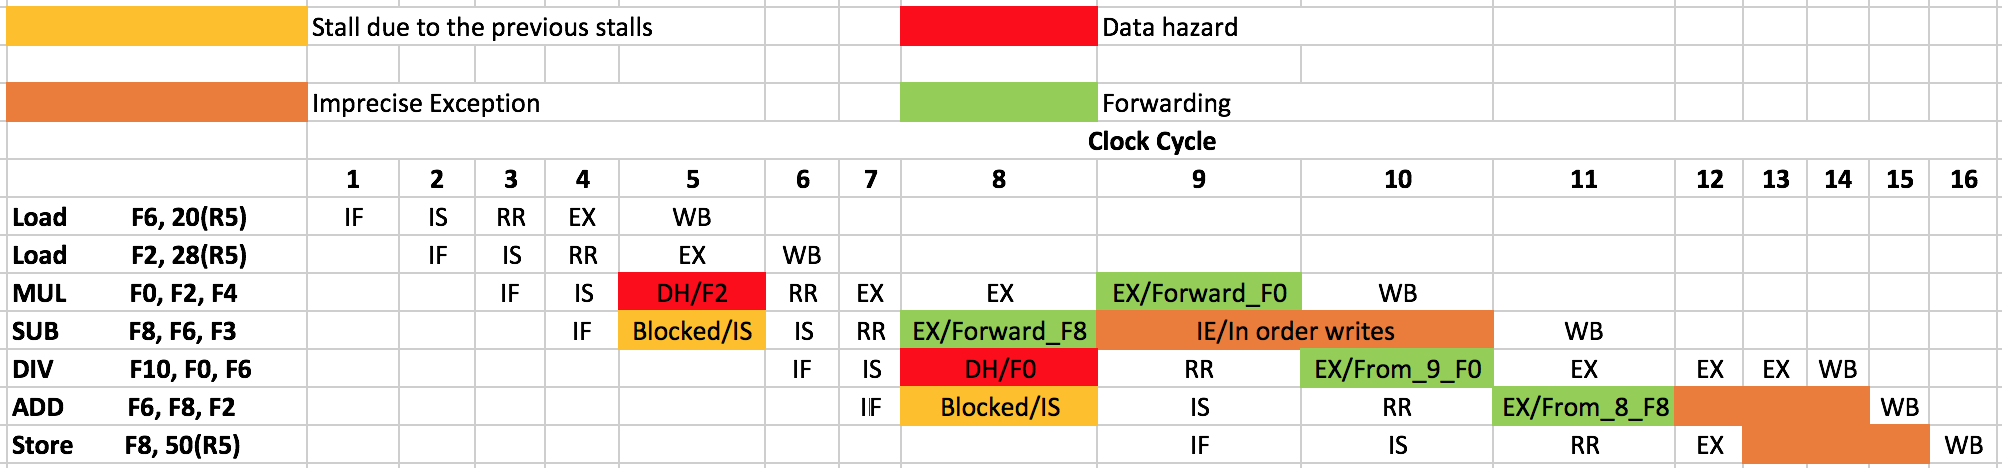
\includegraphics[width=6.8in]{./timediag.PNG}
	\caption{Time Diagram}
	\label{fig:timediag}
\end{figure}


\begin {center}
Load F6, 20(R5) 

Load F2, 28(R5)

MUL F0, F2, F4

SUB F8, F6, F3

DIV F10, F0, F6

ADD F6, F8, F2

Store F8, 50(R5)

\end {center}

\end{enumerate}

\item \textbf{Points of Production and Consumption} n. Consider an un-pipelined processor where it takes 36 ns to go through the circuits and 0.5 ns for the latch overhead. Assume that the point of production and point of consumption in the unpipelined processor are separated by 12 ns. Assume that half the instructions do not introduce a data hazard and half the
instructions depend on their preceding instruction

\begin{enumerate}
\item What is the throughput of the processor with the un-pipelined architecture \textbf{(10 points)}

\fbox{\parbox{5.5in}{
    \textbf{Answer}
    \vspace{0.2in} 
    In un-pipelined architecture, producer/consumer is independent of the time they are separated. Therefore, since every cycle or going through the circuits takes 36$^{ns}$ and 0.5$^{ns}$ of latch overhead, the throughput would be:
     $$\frac{1}{36.5}=27397260$$
    
    }}
	\newline
\item What is the throughput of the processor with a 12-stage pipeline? \textbf {(10 points)}

\fbox{\parbox{5.5in}{
    \textbf{Answer}
    \vspace{0.2in} 
    Every instruction completes in $T=36^{ns}$. So, in a (N=12)-stage pipeline, the time per stage would be:
    $$T_{stage} = \frac{T}{N} + T_{ovh} = \frac{36}{12} + 0.5 = 3.5^{ns}$$
    
    And therefore, every in the pipelined architecture, every instruction could be emitted in $3+0.5 = 3.5^{ns}$, if there was no data dependency. Since according to the given assumptions, half of data are dependent, and the producer and consumer are separated by $T_{PC} = 12^{ns}$, where $PC$ stands for Producer/Consumer, there are 3 ($\frac{T_{PC}}{T_{stage}} = \frac{12}{3.5} = 3.43$) cycles between producer and the consumer. Therefore, at every 5 cycle, 2 instructions will be emitted. So, $IPC = \frac{2}{5}$.
    
    }}
	\newline

\end{enumerate}
\end{enumerate}


\end{document}